% Chapter 1

\chapter{Introduction} % Main chapter title

\label{Chapter1} % For referencing the chapter elsewhere, use \ref{Chapter1} 

\lhead{ \emph{Introduction}} % This is for the header on each page - perhaps a shortened title

%----------------------------------------------------------------------------------------


%----------------------------------------------------------------------------------------






Text mining is used more and more to improve the way we get information or to enhance the way we perceive it. It is incorporated in many fields like politics, social media or improve existing technologies like spam filtering. Text classification is a branch of text mining. It is a classic task in natural language processing. Given a text document and a set of categories, the text classification algorithm must assign the text document into
one or more of the given text categories.\\
Nowadays social networks became a pillar for social interaction and Micro blogging is a new form of communication in which users can describe their current status in short posts distributed by instant messages, mobile phones, email or the Web. Twitter, a popular micro blogging tool has seen a lot of growth since it launched in October, 2006. It helps users to connect with their followers. The tweets from users are referred to as micro blogs because there is a 140 character limit imposed by Twitter for every tweet. This lets the users present any information with only a few words, optionally followed with a link to a more detailed source of information.
The project title in the domain of text classification, more precisely the task of
short text classification, which is more challenging than classic document classification. In
the proposed project title, we use the Twitter Political Corpus"\cite{website:data_set}. Given a tweet, the task
is to distinguish political tweets from non-political ones.

%----------------------------------------------------------------------------------------

% section 1

%----------------------------------------------------------------------------------------
\section{Motivations and goals}
A variety of techniques for supervised learning algorithms have demonstrated reasonable performance for text classification. The question is how would they perform for short text classification.
The project aims to fetch different classification settings, techniques and show how they perform in micro blog text classifications. 
Three different classifiers will be tested: Naïve Bayes, Maximum Entropy and Support Vector Machine.
%----------------------------------------------------------------------------------------

% section 2

%----------------------------------------------------------------------------------------
\section{Outline}
Figure \ref{fig:process_chain} shows the process undertaken in this project.
First we will see how the raw corpus is processed. Then how are the features extraction. Finally the classification results and discussions. 
\begin{figure}[H]
  \centering
  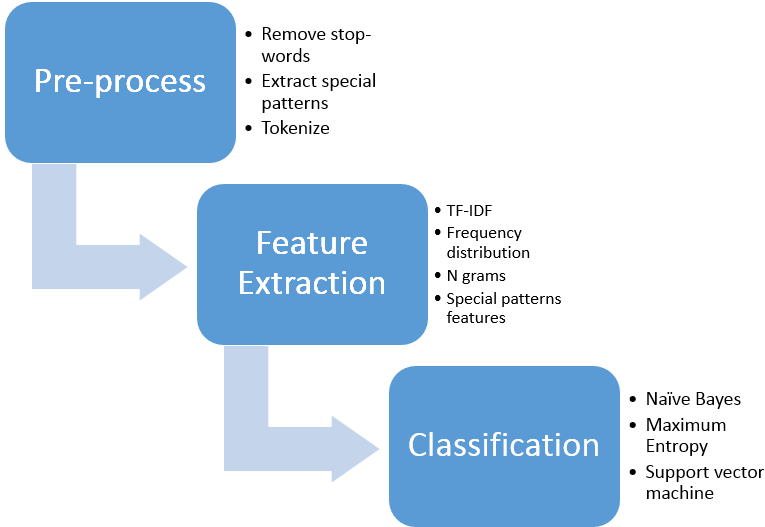
\includegraphics[width=150mm]{figures/process_chain.png}
  \caption{Process chain \label{fig:process_chain}}
\end{figure}